\documentclass[conference]{IEEEtran}
\IEEEoverridecommandlockouts
\usepackage[spanish]{babel}
\usepackage{amsmath,amssymb,amsfonts}
\usepackage{array}     % columnas p{} con \raggedright, para tablas a una columna
\usepackage{graphicx}
\usepackage{textcomp}
\usepackage{listings}
\usepackage{xcolor}
\usepackage{float}
\usepackage{cuted}     % entorno strip: bloque a doble columna que no flota
\usepackage{capt-of}   % \captionof, para rotular dentro de un strip
\usepackage{tcolorbox}
\usepackage{eso-pic}
\usepackage{transparent}
\usepackage{hyperref}  % debe cargarse de último para no duplicar anclas de floats

\pagestyle{plain}

\newif\ifshowwatermark
\showwatermarktrue
\AddToShipoutPictureBG{%
    \ifshowwatermark
        \AtPageCenter{%
            \makebox(0,0){%
                \transparent{0.18}%
                
\includegraphics[width=1.0\textwidth]{assets/images/Logo}%
            }%
        }%
    \fi
}

\lstset{
    language=Python,
    columns=fullflexible,
    basicstyle=\ttfamily\scriptsize\color[RGB]{30,30,30},
    keywordstyle=\bfseries\color[RGB]{0,90,160},
    commentstyle=\itshape\color[RGB]{100,100,100},
    stringstyle=\color[RGB]{160,60,0},
    numberstyle=\tiny\color[RGB]{150,150,150},
    numbers=left,
    numbersep=8pt,
    stepnumber=1,
    backgroundcolor=\color[RGB]{248,248,252},
    frame=none,
    showstringspaces=false,
    breaklines=true,
    breakatwhitespace=false,
    tabsize=4,
    captionpos=b,
    xleftmargin=15pt,
    xrightmargin=5pt,
    inputencoding=utf8,
    extendedchars=true,
    literate=
        {á}{{\'a}}1 {é}{{\'e}}1 {í}{{\'i}}1 {ó}{{\'o}}1 {ú}{{\'u}}1
        {Á}{{\'A}}1 {É}{{\'E}}1 {Í}{{\'I}}1 {Ó}{{\'O}}1 {Ú}{{\'U}}1
        {ñ}{{\~n}}1 {Ñ}{{\~N}}1
        {°}{{\textdegree}}1
        {¨}{}1,
    morekeywords={np, plt, axes, fig}
}

% Estilo específico para los listados de R del Apéndice B.
\lstdefinestyle{Rstyle}{
    language=R,
    morekeywords={png, dev.off, par, boxplot, barplot, legend, grid, points,
                  abline, aggregate, sprintf, file.path, dir.exists, dir.create,
                  read.csv, head, str, plot, pie, text, lm, cor, order, sum, rep, c},
}

% Tabla a doble columna continua a la narrativa: se imprime en el punto exacto
% del texto en lugar de flotar al inicio de la página, como haría table*.
% Las figuras usan figure[H] a una columna, que tampoco flota pero además pasa
% entera a la página siguiente cuando no cabe, en vez de partirse.
\newenvironment{widetable}
    {\begin{strip}\centering}
    {\end{strip}}

\def\BibTeX{{\rm B\kern-.05em{\sc i\kern-.025em b}\kern-.08em T\kern-.1667em\lower.7ex\hbox{E}\kern-.125emX}}

\renewcommand{\refname}{Referencias}

\addto\captionsspanish{%
    \renewcommand{\tablename}{Tabla}%
    \renewcommand{\lstlistingname}{Código}%
}

\begin{document}
    \raggedbottom
    \bstctlcite{IEEEtran:BSTcontrol}

    \title{
        Introducción a la visualización de datos y principios de diseño de gráficos:
        aplicación sobre consumo energético con Matplotlib y R
    }

    \author{\IEEEauthorblockN{
        Andrés Giovanny Rubiano Muñoz ``Andy Rubiano''}
        \IEEEauthorblockA{
            \textit{Maestría en Inteligencia Artificial, Facultad de Ingeniería} \\
            \textit{Universidad de La Salle} \\
            Bogotá, Colombia \\
            arubiano67@unisalle.edu.co
        }
    }

    \maketitle
    \thispagestyle{plain}

    \begin{abstract}
        El presente informe analiza la importancia de la visualización de 
        datos en la ciencia de datos y los principios de diseño que permiten
        diferenciar una representación clara de una potencialmente engañosa,
        tomando como referencia los criterios de Cleveland y McGill, Tufte y 
        Few sobre un conjunto simulado de consumo energético de 120 clientes,
        distribuidos en los sectores Residencial, Comercial e Industrial,
        construyendo cinco visualizaciones en Matplotlib y una representación
        deliberadamente defectuosa, además de replicar cuatro gráficos en R como
        verificación cruzada. Los resultados evidencian una asimetría de 1,85 en
        la distribución del consumo, una relación de 10,7 veces entre el consumo
        industrial y residencial promedio y una correlación de Pearson de 0,998
        entre consumo y costo. Asimismo, el sector Industrial, con el 15\% de
        los clientes, concentra el 48,6\% del consumo total. La comparación
        entre Python y R produjo resultados consistentes, confirmando que la
        calidad de una visualización depende principalmente de sus principios de
        diseño y no de la herramienta utilizada.
    \end{abstract}

    \vspace{10pt}

    \begin{IEEEkeywords}
        Visualización de datos, principios de diseño de gráficos, percepción gráfica,
        canales visuales, integridad gráfica, Matplotlib, R, ciencia de datos.
    \end{IEEEkeywords}

    \section{Introducción}
    Una prueba de hipótesis permite evaluar una afirmación sobre una población 
    a partir de una muestra mediante una hipótesis nula $H_0$ y una alternativa
    $H_1$, la decisión se basa en comparar el valor $p$ con un nivel de
    significancia $\alpha$ fijado previamente, sin embargo, un valor $p$ no 
    indica por sí solo la magnitud del efecto ni permite determinar si la 
    estructura de los datos es adecuada para la conclusión \cite{montgomery2020design},
    \cite{walpole2012probabilidad}, \cite{wasserstein2016asa}.

    \vspace{10pt}

    Esta limitación puede hacerse evidente cuando se combinan observaciones de
    diferentes subpoblaciones. El cuarteto de Anscombe muestra cómo conjuntos con
    estadísticas similares pueden presentar estructuras muy distintas al
    mostrarse de manera gráfica \cite{anscombe1973graphs}. De forma similar, la
    agregación de grupos con comportamientos diferentes puede ocultar o incluso
    modificar una asociación, como ocurre en la paradoja de Simpson
    \cite{kievit2013simpson}, \cite{simpson1951interpretation}, por ello, la
    visualización constituye una herramienta de diagnóstico y no solo un recurso
    para dar a conocer los resultados \cite{few2012show}, 
    \cite{castro2026visualizacion}.

    \vspace{10pt}

    Este informe reproduce este escenario mediante un conjunto simulado de 300
    clientes de los sectores Residencial, Comercial e Industrial, cuyas escalas
    de consumo son diferentes. Se aplican pruebas de hipótesis para comparar
    medias y analizar la relación entre temperatura y consumo, verificando
    previamente sus supuestos. La simulación permite además contrastar los
    resultados obtenidos con las relaciones definidas en los datos.

    \vspace{10pt}

    El análisis se desarrolla en Python con \textit{*SciPy*} y se replica en R,
    acompañando cada prueba con su respectiva visualización. El propósito es
    determinar cuándo un valor $p$ no significativo realmente indica ausencia de
    relación y cuándo una relación puede estar oculta por la estructura de los
    datos, para ello, se contrastan cinco hipótesis, se verifican los supuestos,
    se generan visualizaciones estáticas e interactivas y se interpretan los
    resultados desde una perspectiva estadística y práctica.
    \section{Conceptos fundamentales de la visualización de datos}
\label{fundamentals}
    \subsection{Codificación visual y tipo de variable}
    \label{visual_encoding}
        Toda visualización es una función que asigna valores de datos a atributos
        gráficos que depende del tipo de variable, algunas de ellas son: las variables
        nominales (como el sector del cliente) admiten codificación por posición
        categórica, forma o matiz de color, pero no por longitud continua, las ordinales
        exigen una codificación que preserve el orden y las cuantitativas (consumo en
        kWh, costo en COP) que admiten posición, longitud y área con precisiones muy
        distintas entre sí \cite{castro2026ciencia}.

    \subsection{Jerarquía de precisión de los canales visuales}
    \label{visual_channels}
        El aporte experimental de Cleveland y McGill es la base cuantitativa del diseño
        gráfico moderno, puesto que, al medir el error en la estimación de magnitudes,
        se establece el ordenamiento de precisión decreciente
        \cite{cleveland1984graphical}, el cual se da de la siguiente manera:

        \vspace{10pt}

        \begin{itemize}
            \item Posición sobre una escala común (gráficos de dispersión, barras
            alineadas).

            \item Posición sobre escalas no alineadas (paneles múltiples).

            \item Longitud (barras).

            \item Ángulo y pendiente (gráficos de torta).

            \item Área (burbujas).

            \item Volumen, curvatura y saturación de color.
        \end{itemize}

    \subsection{Correspondencia entre tarea analítica y tipo de gráfico}
    \label{task_chart_correspondence}
        Elegir un tipo de gráfico no es una decisión estética, sino la respuesta a una
        pregunta analítica concreta, ya que no es lo mismo examinar cómo se distribuye
        una variable, que comparar magnitudes entre categorías o buscar la relación
        entre dos medidas, por consiguiente, cada una de estas tareas tiene formas
        gráficas que la responden con mayor precisión que otras, apoyándose en la
        jerarquía de canales visuales descrita en la sección \ref{visual_channels},
        sintetizando dicha correspondencia justificando la elección de la siguiente
        manera:

        \begin{table}[H]
            \centering
            \caption{Correspondencia entre tarea analítica y forma gráfica}
            \begin{center}
                \footnotesize
                \begin{tabular}{|>{\raggedright\arraybackslash}p{1.9cm}|>{\raggedright\arraybackslash}p{1.7cm}|>{\raggedright\arraybackslash}p{2.9cm}|}
                    \hline
                    \textbf{Tarea analítica} & \textbf{Gráfico} & \textbf{Canal y justificación} \\
                    \hline
                    Distribución de una variable & Histograma & Posición y longitud; revela asimetría y multimodalidad \\
                    \hline
                    Comparación entre categorías & Barras & Longitud sobre línea base común desde cero \\
                    \hline
                    Relación entre dos variables & Dispersión & Posición en dos escalas comunes \\
                    \hline
                    Dispersión y atípicos por grupo & Diagrama de caja & Posición; resume cinco estadísticos \\
                    \hline
                    Composición de un total & Barras horizontales ordenadas & Longitud; sustituye al ángulo de la torta \\
                    \hline
                \end{tabular}
                \label{task_chart_mapping}
            \end{center}
        \end{table}
    \section{Principios de diseño de gráficos}
\label{design_principles}
    Los principios que se aplicaron de forma explícita en cada figura provienen
    fundamentalmente de Few \cite{few2012show} y Tufte \cite{tufte2001visual}, los
    cuales son:

    \vspace{10pt}

    \begin{itemize}
        \item \textbf{Integridad gráfica:} la representación visual debe ser
        proporcional a las cantidades que representa, de modo que el factor de mentira
        se mantenga cercano a uno, por ello, las perspectivas tridimensionales, las
        sombras y el desplazamiento radial (\textit{explode}) deben evitarse, ya que
        distorsionan la magnitud visual de los datos
        \cite{few2012show}.

        \item \textbf{Razón dato-tinta:} la mayor parte del gráfico debe destinarse a
        representar datos evitando rejillas gruesas, marcos dobles, fondos y efectos
        decorativos que consumen la atención sin aportar información
        \cite{few2012show}.

        \item \textbf{Etiquetado completo:} todo gráfico debe ser autocontenido, con
        título informativo, ejes rotulados con unidades explícitas y cuando las
        categorías lo permiten, etiquetas numéricas directas \cite{few2012show}.

        \item \textbf{Uso funcional del color:} el color codifica información, no
        decora, puesto que los matices se reservan para las variables nominales, las
        escalas secuenciales para las cuantitativas y si solo hay una variable, se
        prefiere un color único \cite{few2012show}.

        \item \textbf{Escala honesta:} en los gráficos de barras el eje parte de cero,
        porque se compara por longitud; en los de dispersión es legítimo truncar el
        rango, porque se lee por posición relativa \cite{few2012show}.

        \item \textbf{Ordenamiento significativo:} cuando la categoría no tiene orden
        natural, organizarla por magnitud reduce el esfuerzo de comparación visual del
        lector \cite{few2012show}.

        \item \textbf{Jerarquía visual:} la cuadrícula y los ejes se dibujan por detrás
        de los datos y con menor peso visual, dejando la información en primer plano
        \cite{few2012show}.
    \end{itemize}
    \section{Comparación de herramientas de visualización}
\label{tools_comparison}
    \subsection{Panorama de herramientas}
    \label{tools_overview}
        Las herramientas de visualización pueden organizarse en cuatro enfoques,
        cada uno con un equilibrio distinto entre control, facilidad de uso,
        interactividad y reproducibilidad. El enfoque imperativo construye la 
        figura instrucción por instrucción y ofrece un control detallado sobre 
        cada elemento, en este grupo, Matplotlib proporciona gráficos de alta 
        resolución y una licencia libre, aunque requiere más código, de forma 
        similar, la graficación base de R funciona sin dependencias, pero ofrece 
        una composición por capas menos flexible \cite{castro2026ciencia}, 
        \cite{wilkinson2005grammar}, \cite{hunter2007matplotlib}. El enfoque 
        declarativo, inspirado en la gramática de gráficos de Wilkinson, 
        permite describir qué se desea mostrar y delega el trazado en la 
        herramienta, por ello, \textit{seaborn}, \textit{ggplot2} y 
        \textit{Altair} producen gráficos estadísticos expresivos con pocas 
        líneas de código, aunque con menor control sobre los detalles más 
        finos \cite{wilkinson2005grammar}. En el ámbito web, \textit{Plotly} 
        y \textit{D3.js} añaden interactividad de forma nativa, pero su desarrollo 
        suele requerir un esfuerzo mayor \cite{castro2026ciencia}. Finalmente, 
        las herramientas de interfaz gráfica reemplazan el código por la
        manipulación directa de los elementos, como es el caso de \textit{Tableau} 
        y \textit{Power BI} que permiten construir tableros rápidamente y 
        cuentan con una amplia adopción empresarial, sin embargo, ofrecen menor 
        reproducibilidad y requieren licencias comerciales \cite{castro2026ciencia}, 
        \cite{hunter2007matplotlib}.

    \subsection{Elección de herramientas: Matplotlib y R}
    \label{tools_choice}
        En Python se selecciona Matplotlib porque permite un mayor control sobre 
        los elementos de la figura, como la cuadrícula, las etiquetas y los ejes
        \cite{castro2026ciencia}, además, bibliotecas como \textit{seaborn} y el 
        método \texttt{DataFrame.plot} de \textit{pandas} utilizan Matplotlib 
        como base, por lo que su dominio facilita el uso de estas herramientas
        \cite{hunter2007matplotlib}. Su integración con \textit{pandas} y
        \textit{NumPy} también permite realizar los cálculos y generar las
        visualizaciones dentro de un mismo script reproducible, utilizando 
        funcionalidades de código abierto y sin costo \cite{mckinney2010data}, 
        \cite{harris2020array}. Por el lado de R, se utiliza la graficación base 
        como herramienta de contraste, pues repetir los mismos cálculos y 
        visualizaciones en un lenguaje diferente permite comprobar que los 
        principios de diseño no dependen de una herramienta específica y 
        ayuda a identificar posibles errores de implementación en cualquiera de 
        los dos entornos \cite{castro2026ciencia}.

    \section{Metodología}
    El desarrollo se implementó en dos scripts independientes: \textit{Python}
    genera el conjunto de datos, ejecuta las cinco pruebas y produce las figuras;
    \textit{R} lee el mismo archivo y recalcula todo desde cero, de modo que
    cualquier discrepancia delataría un error de implementación. El núcleo
    estadístico de ambos se reproduce en los Anexos \ref{anexo_python} y
    \ref{anexo_r}. Todas las pruebas usan $\alpha = 0{,}05$.

    \subsection{Conjunto de datos}
        Se emplea un conjunto simulado de consumo energético mensual de 300
        clientes, 100 por cada sector, generado con semilla fija (42) para
        garantizar la reproducibilidad. Las variables se resumen en la Tabla
        \ref{dataset_variables}.

        \begin{table}[H]
            \centering
            \caption{Variables del conjunto de datos}
            \begin{center}
                \begin{tabular}{|l|l|>{\raggedright\arraybackslash}p{2.9cm}|}
                    \hline
                    \textbf{Variable} & \textbf{Tipo} & \textbf{Descripción} \\
                    \hline
                    id\_cliente & Nominal & Identificador único
                    (CL-0001 a CL-0300) \\
                    \hline
                    sector & Nominal & Residencial, Comercial o Industrial \\
                    \hline
                    region & Nominal & Andina, Caribe o Pacífica \\
                    \hline
                    temperatura\_c & Continua & Temperatura promedio del mes
                    en \textdegree C \\
                    \hline
                    consumo\_kwh & Continua & Consumo mensual en
                    kilovatios-hora \\
                    \hline
                \end{tabular}
                \label{dataset_variables}
            \end{center}
        \end{table}

        El consumo se construye según la ecuación (\ref{generador}), donde
        $\mu_s$ y $\sigma_s$ son la media y la desviación propias de cada sector y
        $T_i$ la temperatura del cliente, cuya región se asigna con independencia
        del sector.

        \begin{equation}
            Y_i = \mathcal{N}(\mu_s, \sigma_s^2) + 4\,(T_i - 20)
            \label{generador}
        \end{equation}

        El coeficiente 4 es el dato decisivo del experimento: la relación
        temperatura consumo existe por diseño, es idéntica en los tres sectores y
        su magnitud se conoce de antemano, lo que convierte al conjunto en un banco
        de pruebas donde puede verificarse qué recupera cada estadístico. Los
        sectores, en cambio, se separan por niveles muy distintos, con medias de
        180, 420 y 900 kWh y desviaciones de 40, 90 y 180 kWh respectivamente.

    \subsection{Diseño del contraste}
        Las cinco hipótesis se resumen en la Tabla \ref{hipotesis}. Las dos primeras
        no son un trámite previo sino que condicionan a las siguientes, ya que
        determinan si las pruebas paramétricas son aplicables y bajo qué variante.

        \begin{table}[H]
            \centering
            \caption{Hipótesis contrastadas e implementación}
            \begin{center}
                \begin{tabular}{|c|>{\raggedright\arraybackslash}p{2.4cm}|l|l|}
                    \hline
                    \textbf{\#} & \textbf{Hipótesis nula} & \textbf{Python} &
                    \textbf{R} \\
                    \hline
                    1 & El consumo de cada sector es normal & \texttt{shapiro} &
                    \texttt{shapiro.test} \\
                    \hline
                    2 & Las varianzas son homogéneas & \texttt{levene} &
                    \texttt{bartlett.test} \\
                    \hline
                    3 & $\mu_{Res} = \mu_{Com}$ & \texttt{ttest\_ind} &
                    \texttt{t.test} \\
                    \hline
                    4 & $\mu_{Res} = \mu_{Com} = \mu_{Ind}$ & \texttt{anova\_lm} &
                    \texttt{aov} \\
                    \hline
                    5 & $\rho_{T,Y} = 0$ & \texttt{pearsonr} &
                    \texttt{cor.test} \\
                    \hline
                \end{tabular}
                \label{hipotesis}
            \end{center}
        \end{table}

        La comparación de dos medias emplea el estadístico de la ecuación
        (\ref{welch}), que no asume varianzas iguales y ajusta los grados de
        libertad mediante la aproximación de Welch-Satterthwaite
        \cite{welch1947generalization}.

        \begin{equation}
            t = \frac{\bar{x}_1 - \bar{x}_2}
                     {\sqrt{\dfrac{s_1^2}{n_1} + \dfrac{s_2^2}{n_2}}}
            \label{welch}
        \end{equation}

        Para tres o más grupos se recurre al ANOVA de un factor, cuyo estadístico
        de la ecuación (\ref{anova}) contrasta la variabilidad entre grupos frente
        a la que existe dentro de ellos \cite{montgomery2020design}.

        \begin{equation}
            F = \frac{SC_{entre} / (k-1)}{SC_{dentro} / (N-k)}
            \label{anova}
        \end{equation}

        Un $F$ significativo indica que al menos una media difiere, pero no cuál,
        por lo que se aplica el post-hoc de Tukey de la ecuación (\ref{tukey}), que
        controla la tasa de error por familia al examinar las tres comparaciones
        por pares \cite{tukey1949comparing}.

        \begin{equation}
            HSD = q_{\alpha,k,N-k} \sqrt{\frac{CM_{dentro}}{n}}
            \label{tukey}
        \end{equation}

        Por último, la relación entre temperatura y consumo se evalúa con el
        coeficiente de Pearson de la ecuación (\ref{pearson})
        \cite{pearson1895regression} y con la recta de regresión estimada por
        mínimos cuadrados de la ecuación (\ref{ols}).

        \begin{equation}
            r = \frac{\sum (T_i - \bar{T})(Y_i - \bar{Y})}
                     {\sqrt{\sum (T_i - \bar{T})^2 \sum (Y_i - \bar{Y})^2}}
            \label{pearson}
        \end{equation}

        \begin{equation}
            \hat{Y} = b_0 + b_1 T
            \label{ols}
        \end{equation}

        Ambas cantidades se calculan a nivel global y, de forma separada, dentro de
        cada sector. Esa doble mirada es la que permite detectar el efecto de la
        agregación que se analiza en la Sección \ref{seccion_visualizacion}.

    \subsection{Magnitud del efecto y potencia}
        \label{subsec_efecto}
        Un valor $p$ responde si una diferencia es distinguible del azar, no si
        importa; con $n = 100$ por grupo casi cualquier separación alcanza la
        significancia, de modo que reportar únicamente el valor $p$ reproduce el
        problema que advierte la declaración de la ASA \cite{wasserstein2016asa}.
        Cada contraste se acompaña por ello de su tamaño de efecto
        \cite{cohen1988statistical}, \cite{lakens2013calculating}. Para la
        comparación de dos medias se emplea la $d$ de Cohen de la ecuación
        (\ref{cohend}), con $s_p$ la desviación combinada, y su corrección de
        sesgo $g$ de Hedges.

        \begin{equation}
            d = \frac{\bar{x}_1 - \bar{x}_2}{s_p}, \qquad
            s_p = \sqrt{\frac{(n_1-1)s_1^2 + (n_2-1)s_2^2}{n_1 + n_2 - 2}}
            \label{cohend}
        \end{equation}

        Para el ANOVA se reportan la proporción de varianza explicada $\eta^2$ y
        su versión corregida $\omega^2$ de la ecuación (\ref{omega}), que
        descuenta el sesgo optimista de la primera.

        \begin{equation}
            \eta^2 = \frac{SC_{entre}}{SC_{total}}, \qquad
            \omega^2 = \frac{SC_{entre} - (k-1)\,CM_{dentro}}
                            {SC_{total} + CM_{dentro}}
            \label{omega}
        \end{equation}

        La potencia observada se calcula sobre la distribución no central
        correspondiente a cada estadístico. A ella se añade un análisis de
        sensibilidad sobre la quinta hipótesis: la correlación más pequeña
        detectable con potencia $1-\beta = 0{,}80$ y $n$ observaciones se obtiene
        invirtiendo la transformación de Fisher según la ecuación
        (\ref{rdetectable}). Ese umbral separa dos explicaciones posibles de una
        correlación no significativa, la falta de tamaño muestral y la pequeñez
        real del coeficiente.

        \begin{equation}
            r_{\min} = \tanh\!\left(\frac{z_{1-\alpha/2} + z_{1-\beta}}
                                         {\sqrt{n-3}}\right)
            \label{rdetectable}
        \end{equation}

    \subsection{Contrastes robustos a la heterocedasticidad}
        \label{subsec_robustez}
        Tanto el ANOVA clásico como el post-hoc de Tukey asumen varianzas
        iguales, supuesto que la segunda hipótesis rechaza. En lugar de dejar
        constancia de ello como una limitación, todo el bloque de comparación de
        medias se repite con los procedimientos que no lo exigen: el ANOVA de
        Welch de la ecuación (\ref{welchanova}), que pondera cada grupo por
        $w_i = n_i/s_i^2$ \cite{welch1951comparison}, y el post-hoc de
        Games-Howell de la ecuación (\ref{gameshowell}), que sustituye el error
        estándar común de Tukey por el de Welch en cada par y ajusta los grados
        de libertad mediante Welch-Satterthwaite \cite{games1976pairwise}.

        \begin{equation}
            F_W = \frac{\dfrac{1}{k-1}\sum w_i (\bar{x}_i - \bar{x}_w)^2}
                       {1 + \dfrac{2(k-2)}{k^2-1}\,\Lambda}
            \label{welchanova}
        \end{equation}

        \begin{equation}
            q_{ij} = \frac{|\bar{x}_i - \bar{x}_j|}
                          {\sqrt{\dfrac{1}{2}\left(\dfrac{s_i^2}{n_i}
                                 + \dfrac{s_j^2}{n_j}\right)}}
            \label{gameshowell}
        \end{equation}

        Si ambos procedimientos conducen a la misma decisión, la conclusión queda
        respaldada con independencia del supuesto; si divergieran, habría que
        reportar la versión robusta. El resultado de esa comprobación se presenta
        en la Sección \ref{subsec_robustez_resultados}.

    \subsection{Plan de visualización}
        \label{subsec_plan_visual}
        Cada hipótesis contrastada tiene asignada al menos una figura, y cada
        figura lleva impreso el estadístico y el valor $p$ que representa, de modo
        que pueda leerse sin emparejarla con la tabla correspondiente. Las nueve
        figuras se construyen dos veces, en Python y en R, sobre estadísticos
        calculados de forma independiente en cada entorno. La Tabla
        \ref{plan_figuras} resume esa correspondencia entre hipótesis, biblioteca
        y figura.

        \begin{table}[H]
            \centering
            \caption{Correspondencia entre hipótesis, biblioteca y figura}
            \begin{center}
                \begin{tabular}{|c|>{\raggedright\arraybackslash}p{2.05cm}|l|c|}
                    \hline
                    \textbf{\#} & \textbf{Figura} & \textbf{Biblioteca} &
                    \textbf{Ref.} \\
                    \hline
                    1 & Histograma con normal teórica & Matplotlib / ggplot2 &
                    \ref{fig_normalidad} \\
                    \hline
                    1 & Q-Q por sector & Matplotlib / ggplot2 &
                    \ref{fig_qq} \\
                    \hline
                    2 & Violín con caja y puntos & seaborn / ggplot2 &
                    \ref{fig_boxplot} \\
                    \hline
                    3 & Medias con IC del 95\,\% & Matplotlib / ggplot2 &
                    \ref{fig_medias} \\
                    \hline
                    4 & Forest de Tukey y Games-Howell & Matplotlib / ggplot2 &
                    \ref{fig_forest} \\
                    \hline
                    5 & Dispersión global con recta OLS & seaborn / ggplot2 &
                    \ref{fig_regresion} \\
                    \hline
                    5 & Dispersión por sector \textbf{interactiva} &
                    Plotly / ggplotly & \ref{fig_plotly} \\
                    \hline
                    5 & Descomposición de la atenuación & seaborn / ggplot2 &
                    \ref{fig_atenuacion} \\
                    \hline
                    1--5 & \textbf{Dashboard} de cuatro paneles
                    \textbf{interactivo} & Plotly / ggplotly &
                    \ref{fig_dashboard} \\
                    \hline
                \end{tabular}
                \label{plan_figuras}
            \end{center}
        \end{table}

        Las dos figuras interactivas se exportan como HTML autónomo, junto a sus 
        equivalentes de R generados con \texttt{ggplotly}.
        En ellas la interacción cumple una función analítica y no decorativa: aislar
        un sector desde la leyenda equivale a ejecutar el análisis condicionado que
        sostiene el argumento de este informe, y el \textit{hover} identifica
        cliente y región sin volver a los datos.

    \section{Resultados}
    \subsection{Verificación de supuestos}
        La Tabla \ref{supuestos} resume las dos primeras hipótesis. Los tres sectores 
        cumplen el supuesto de normalidad, lo que permite emplear pruebas paramétricas, 
        en cambio, la homogeneidad de varianzas se rechaza de forma contundente.

        \begin{table}[H]
            \centering
            \caption{Normalidad y homogeneidad de varianzas}
            \begin{center}
                \begin{tabular}{|l|l|c|c|}
                    \hline
                    \textbf{Prueba} & \textbf{Grupo} & \textbf{Estadístico} &
                    \textbf{$p$} \\
                    \hline
                    Shapiro-Wilk & Residencial & 0,9912 & 0,7628 \\
                    \hline
                    Shapiro-Wilk & Comercial   & 0,9868 & 0,4246 \\
                    \hline
                    Shapiro-Wilk & Industrial  & 0,9933 & 0,9069 \\
                    \hline
                    Levene (Python)  & Los 3 sectores & 60,43  & $<0{,}001$ \\
                    \hline
                    Bartlett (R)     & Los 3 sectores & 199,39 & $<0{,}001$ \\
                    \hline
                \end{tabular}
                \label{supuestos}
            \end{center}
        \end{table}

        La heterocedasticidad se evidencia en el aumento de la desviación 
        estándar, de 40,6 kWh en Residencial a 195,3 kWh en Industrial, 
        por ello, la comparación de medias se realiza mediante la corrección 
        de Welch.

        \begin{figure}[H]
            \centering
            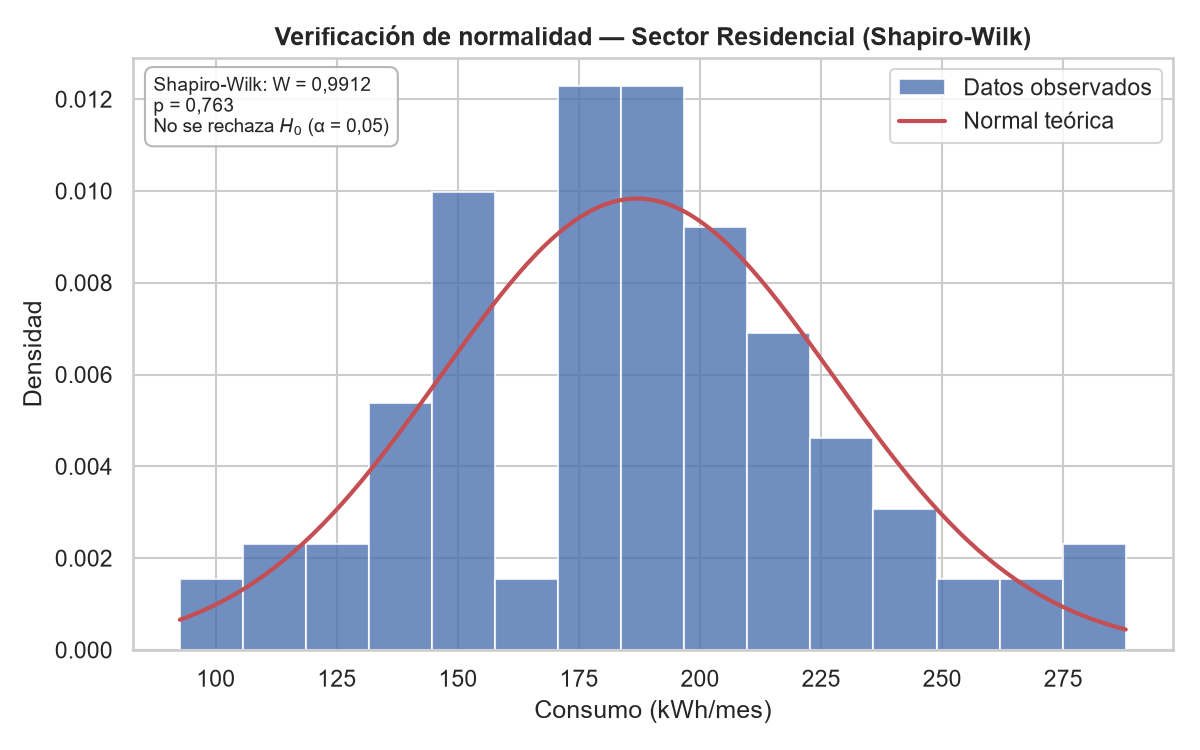
\includegraphics[width=0.99\linewidth]{assets/images/figures/python/hypothesis/histograma_normalidad.png}
            \caption{Verificación de normalidad del sector Residencial: histograma
            de la muestra con la densidad normal teórica superpuesta (Matplotlib)}
            \label{fig_normalidad}
        \end{figure}

        La Figura \ref{fig_normalidad} muestra un comportamiento compatible con 
        la normalidad. El valor $p=0,7628$ sin rechazar $H_0$, mientras 
        que la correspondencia entre el histograma y la distribución normal teórica 
        respalda gráficamente este resultado.

        \begin{strip}
            \centering
            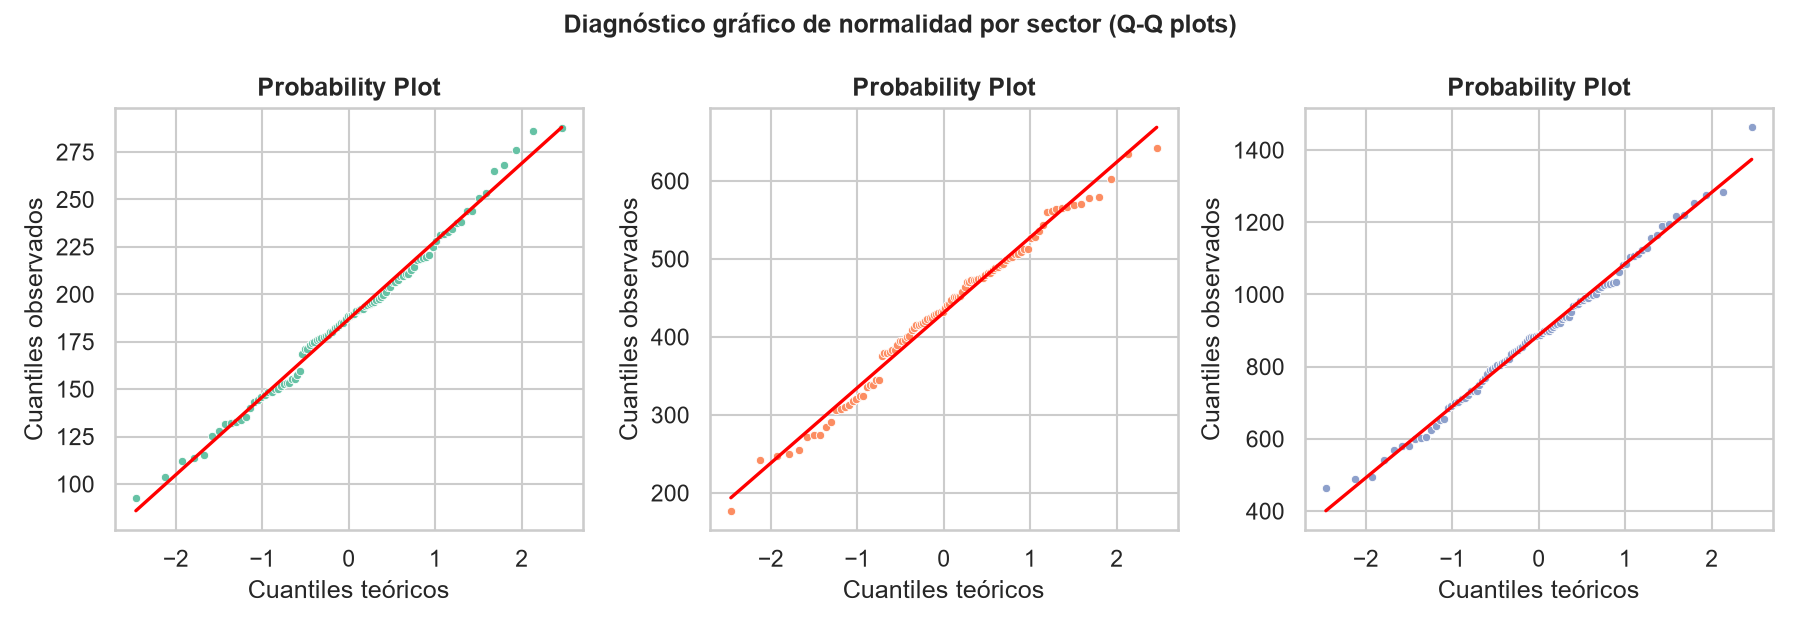
\includegraphics[width=0.92\linewidth]{assets/images/figures/python/hypothesis/qqplots_normalidad.png}
            \captionof{figure}{Diagnóstico gráfico de normalidad en los tres sectores mediante
            gráficos cuantil-cuantil (Matplotlib). Cada panel rotula el estadístico
            $W$ de Shapiro-Wilk y su valor $p$}
            \label{fig_qq}
        \end{strip}

        \clearpage

        El histograma representa el centro de la distribución, pero la
        Figura \ref{fig_qq} permite evaluar mejor las colas. En los tres
        sectores, los puntos siguen la diagonal teórica sin evidenciar asimetría
        ni colas pesadas, respaldando la normalidad tanto gráfica como
        analíticamente \cite{shapiro1965analysis}.

    \subsection{Comparación de medias}
        La Tabla \ref{ttest} compara el consumo promedio de dos sectores, el
        Residencial consume \textbf{187 kWh} al mes, mientras que el Comercial
        consume \textbf{431 kWh}, es decir, más del doble. Este salto de 244 kWh
        es tan consistente que ningún cliente residencial típico se parece a 
        ningún cliente comercial típico. El valor $p < 10^{-49}$ (prácticamente 
        cero) niega cualquier posibilidad de que esta diferencia sea fruto del 
        azar.

        \begin{table}[H]
            \centering
            \caption{Prueba t de Welch: Residencial vs. Comercial}
            \begin{center}
                \begin{tabular}{|l|c|c|c|c|c|}
                    \hline
                    \textbf{Grupo} & \textbf{$n$} & \textbf{Media} &
                    \textbf{$s$} & \textbf{$t$} & \textbf{$p$} \\
                    \hline
                    Residencial & 100 & 186,98 & 40,57 & \multirow{2}{*}{$-23{,}54$}
                    & \multirow{2}{*}{$2{,}3\times10^{-49}$} \\
                    \cline{1-4}
                    Comercial   & 100 & 431,30 & 95,54 & & \\
                    \hline
                \end{tabular}
                \label{ttest}
            \end{center}
        \end{table}

        Extendiendo el análisis a los tres sectores (Residencial, Comercial e
        Industrial), el ANOVA de la Tabla \ref{anova_tabla} rechaza la hipótesis
        de que consuman lo mismo. El estadístico $F=775,99$ es extremadamente
        grande e indica que la variabilidad entre sectores es 776 veces más 
        grande que la variabilidad dentro de cada sector. Con
        $p < 10^{-118}$, concluyendo que el sector determina el consumo.

        \begin{table}[H]
            \centering
            \caption{ANOVA de un factor sobre el consumo}
            \begin{center}
                \begin{tabular}{|l|c|c|c|c|}
                    \hline
                    \textbf{Fuente} & \textbf{SC} & \textbf{gl} & \textbf{$F$} &
                    \textbf{$p$} \\
                    \hline
                    Sector   & 25.298.262,0 & 2   & 775,99 &
                    $1{,}2\times10^{-118}$ \\
                    \hline
                    Residual & 4.841.297,4  & 297 & & \\
                    \hline
                \end{tabular}
                \label{anova_tabla}
            \end{center}
        \end{table}

        El sector explica el \textbf{83,9\%} de la variabilidad total del
        consumo, lo que evidencia una fuerte diferenciación entre los grupos 
        y el 16,1\% restante corresponde a variaciones individuales dentro de 
        cada sector. Esta alta proporción anticipa un aspecto relevante del 
        análisis posterior, porque al concentrar el sector y la mayor parte de 
        la variabilidad, otros factores pueden quedar parcialmente ocultos.

        \begin{table}[H]
            \centering
            \caption{Comparaciones múltiples de Tukey (IC del 95\,\%)}
            \begin{center}
                \begin{tabular}{|l|r|c|c|}
                    \hline
                    \textbf{Comparación} & \textbf{Dif.} & \textbf{IC 95\,\%}
                    & \textbf{$p$ ajust.} \\
                    \hline
                    Ind. $-$ Com. & $+456{,}4$ & [413,8 ; 498,9] &
                    $<0{,}001$ \\
                    \hline
                    Res. $-$ Com. & $-244{,}3$ & [$-286{,}9$ ; $-201{,}8$] &
                    $<0{,}001$ \\
                    \hline
                    Res. $-$ Ind. & $-700{,}7$ & [$-743{,}2$ ; $-658{,}2$] &
                    $<0{,}001$ \\
                    \hline
                \end{tabular}
                \label{tukey_tabla}
            \end{center}
        \end{table}

        El post-hoc de la Tabla \ref{tukey_tabla} confirma que las tres
        comparaciones son significativas y que ningún par de sectores 
        puede tratarse como equivalente. Las Figuras \ref{fig_boxplot} y 
        \ref{fig_medias} traducen ambas tablas: la primera muestra cajas 
        sin traslape con amplitudes crecientes, que sostienen a la vez el 
        rechazo del ANOVA y el de la homogeneidad de varianzas; la segunda 
        convierte el resultado de Tukey en intervalos de confianza que no 
        se solapan.

        \begin{figure}[H]
            \centering
            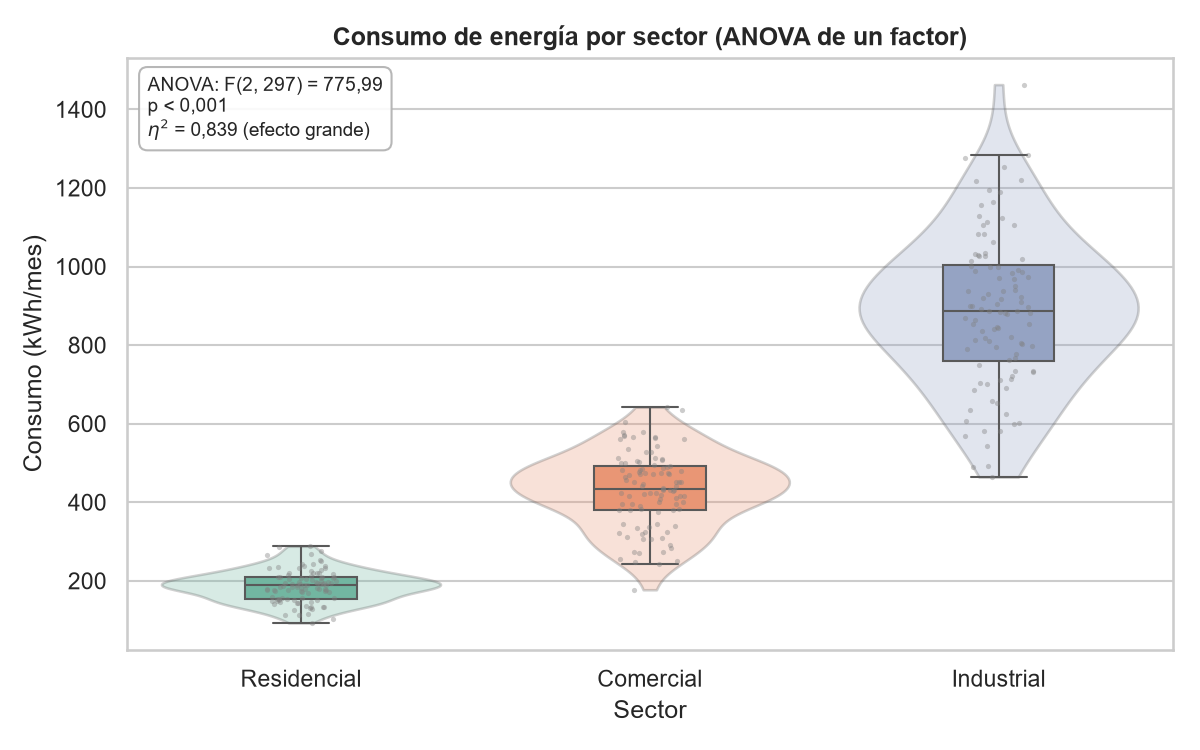
\includegraphics[width=1\linewidth]{assets/images/figures/python/hypothesis/boxplot_sectores.png}
            \caption{Distribución del consumo por sector: violín, caja e
            individuos superpuestos, con el resultado del ANOVA y su $\eta^2$
            rotulados sobre la propia figura (seaborn)}
            \label{fig_boxplot}
        \end{figure}

        \begin{figure}[H]
            \centering
            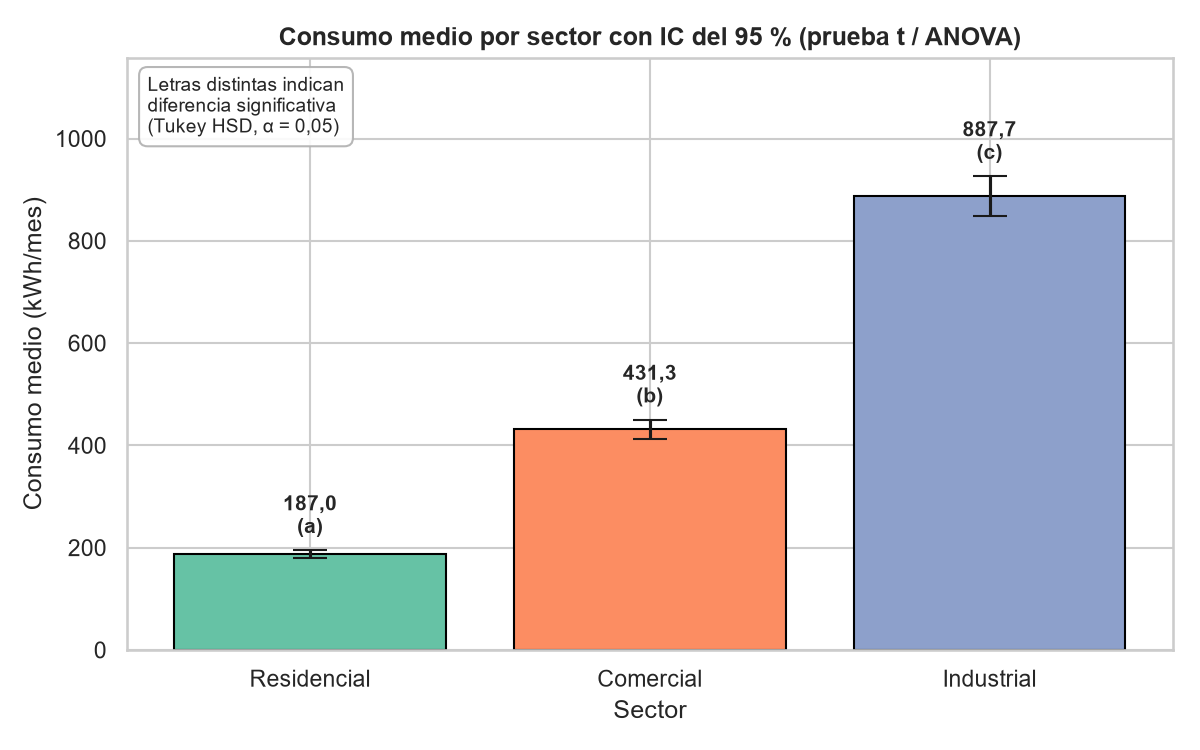
\includegraphics[width=1\linewidth]{assets/images/figures/python/hypothesis/medias_ic95.png}
            \caption{Consumo medio por sector con intervalos de confianza del
            95\,\%. Las letras (a), (b) y (c) codifican el post-hoc de Tukey:
            sectores con letras distintas difieren significativamente (Matplotlib)}
            \label{fig_medias}
        \end{figure}

    \subsection{Magnitud del efecto y potencia}
        \label{subsec_efecto_resultados}
        Los valores $p$ de las Tablas \ref{ttest} y \ref{anova_tabla} son tan
        extremos que dejan de ser informativos, con $n = 100$ por grupo indican
        que la diferencia existe, pero no cuánto vale. La Tabla \ref{efectos}
        cuantifica esa magnitud.

        \begin{table}[H]
            \centering
            \caption{Tamaños de efecto y potencia observada}
            \begin{center}
                \begin{tabular}{|>{\raggedright\arraybackslash}p{2.35cm}|c|c|l|}
                    \hline
                    \textbf{Medida} & \textbf{Valor} & \textbf{IC 95\,\%} &
                    \textbf{Lectura} \\
                    \hline
                    $d$ de Cohen (Res.--Com.) & 3,329 & [2,901 ; 3,757] &
                    Muy grande \\
                    \hline
                    $g$ de Hedges & 3,316 & --- & Muy grande \\
                    \hline
                    $\eta^2$ (sector) & 0,839 & --- & Muy grande \\
                    \hline
                    $\omega^2$ (sector) & 0,838 & --- & Muy grande \\
                    \hline
                    $f$ de Cohen (sector) & 2,286 & --- & Muy grande \\
                    \hline
                    Potencia ($t$ de Welch) & $>0{,}999$ & --- & Máxima \\
                    \hline
                    Potencia (ANOVA) & $>0{,}999$ & --- & Máxima \\
                    \hline
                \end{tabular}
                \label{efectos}
            \end{center}
        \end{table}

        Una $d=3,33$ indica una diferencia superior a tres desviaciones
        típicas entre Residencial y Comercial, muy por encima del umbral de
        efecto grande de 0,80 propuesto por Cohen \cite{cohen1988statistical}.
        El intervalo de confianza respalda esta magnitud y la corrección de
        Hedges apenas modifica la estimación. Asimismo, $\omega^2=0{,}838$ es
        prácticamente igual a $\eta^2=0{,}839$, lo que confirma que el 83,8\% de la
        varianza explicada no se debe al número de grupos. En conjunto, estos
        resultados evidencian un efecto genuinamente grande, no solo un
        resultado asociado al tamaño muestral.

        \vspace{10pt}

        Esta distinción se evidencia en la quinta hipótesis, donde con
        $n=300$ la ecuación (\ref{rdetectable}) establece $r_{\min}=0{,}161$
        como la correlación mínima detectable con una potencia del 80\%. El
        coeficiente global observado ($r=0,063$) queda por debajo de este umbral,
        mientras que el de Residencial ($r=0,595$) lo supera ampliamente, por
        tanto, la no significancia global no responde a un tamaño muestral
        insuficiente, sino a la baja magnitud de la correlación.

    \subsection{Robustez ante la heterocedasticidad}
        \label{subsec_robustez_resultados}
        El ANOVA de la Tabla \ref{anova_tabla} y el post-hoc de Tukey asumen
        varianzas iguales, supuesto que la Tabla \ref{supuestos} rechaza. La
        Tabla \ref{robustez} repite ambos contrastes con los procedimientos que
        no lo exigen.

        \begin{table}[H]
            \centering
            \caption{Contraste clásico frente a su versión robusta}
            \begin{center}
                \begin{tabular}{|l|c|c|c|}
                    \hline
                    \textbf{Procedimiento} & \textbf{$F$ / dif.} &
                    \textbf{gl} & \textbf{$p$} \\
                    \hline
                    ANOVA clásico & 775,99 & 2 ; 297 & $<0{,}001$ \\
                    \hline
                    ANOVA de Welch & 830,22 & 2 ; 156,1 & $<0{,}001$ \\
                    \hline
                    Tukey: Ind.$-$Res. & $+700{,}70$ & 297 & $<0{,}001$ \\
                    \hline
                    G.-Howell: Ind.$-$Res. & $+700{,}70$ & 107,5 & $<0{,}001$ \\
                    \hline
                    Tukey: Com.$-$Res. & $+244{,}33$ & 297 & $<0{,}001$ \\
                    \hline
                    G.-Howell: Com.$-$Res. & $+244{,}33$ & 133,6 & $<0{,}001$ \\
                    \hline
                    Tukey: Ind.$-$Com. & $+456{,}37$ & 297 & $<0{,}001$ \\
                    \hline
                    G.-Howell: Ind.$-$Com. & $+456{,}37$ & 143,8 & $<0{,}001$ \\
                    \hline
                \end{tabular}
                \label{robustez}
            \end{center}
        \end{table}

        La Figura \ref{fig_forest} muestra que Games-Howell estrecha el intervalo 
        entre Comercial y Residencial, pero lo amplía en las comparaciones con
        Industrial, el grupo más disperso. Tukey, al asumir un error estándar
        común, sobreestima la incertidumbre en la primera comparación y la
        subestima en las otras dos.

        \begin{figure}[H]
            \centering
            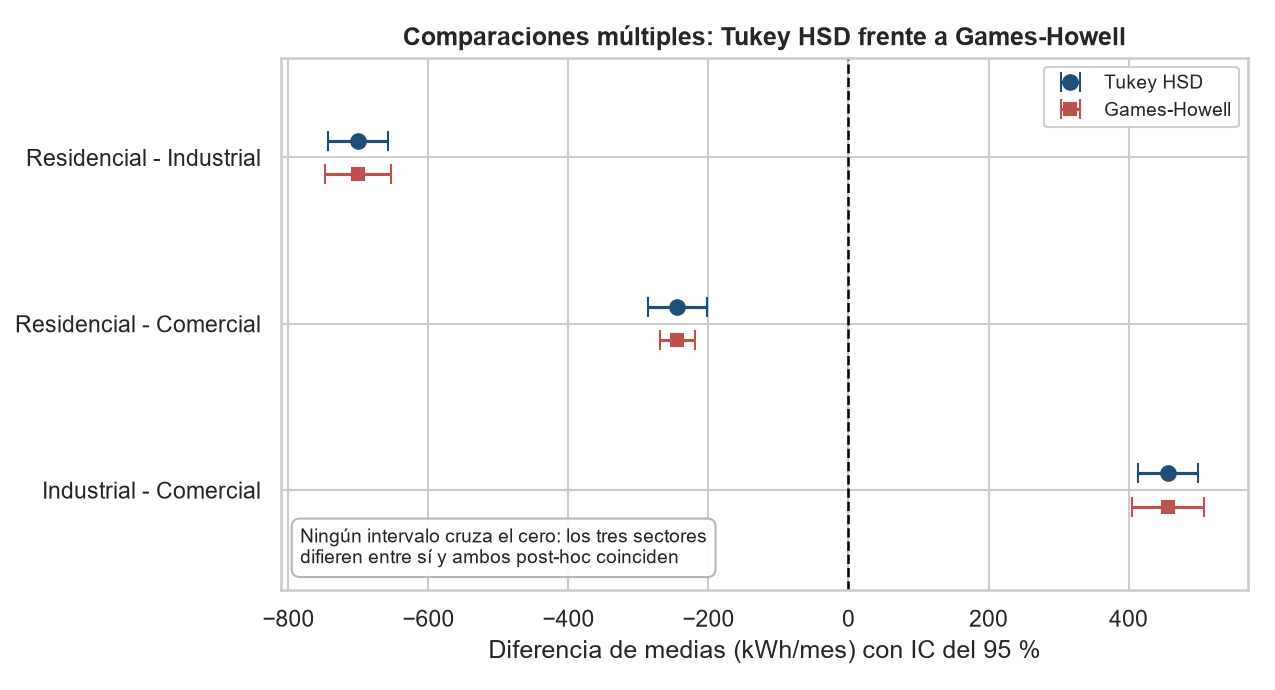
\includegraphics[width=1\linewidth]{assets/images/figures/python/hypothesis/tukey_forest.png}
            \caption{Comparaciones múltiples por pares: intervalos de confianza
            del 95\,\% de Tukey HSD frente a Games-Howell (Matplotlib)}
            \label{fig_forest}
        \end{figure}

        El ANOVA de Welch rechaza la igualdad de medias con un estadístico incluso 
        mayor que el clásico y las tres comparaciones de Games-Howell siguen siendo 
        significativas con intervalos que no cruzan el cero. El rechazo de la 
        homocedasticidad afecta a la precisión de cada intervalo, no a la decisión, 
        de modo que los resultados de las Tablas \ref{anova_tabla} y \ref{tukey_tabla} 
        pueden sostenerse tal como se reportan.

    \subsection{Relación entre temperatura y consumo}
        \label{seccion_regresion}
        La Tabla \ref{correlacion} presenta el coeficiente de Pearson calculado sobre 
        el conjunto completo y por separado, dentro de cada sector.

        \begin{table}[H]
            \centering
            \caption{Correlación temperatura-consumo por ámbito}
            \begin{center}
                \begin{tabular}{|l|c|c|c|l|}
                    \hline
                    \textbf{Ámbito} & \textbf{$n$} & \textbf{$r$} & \textbf{$p$} &
                    \textbf{Decisión} \\
                    \hline
                    Global      & 300 & 0,063 & 0,277 & No se rechaza $H_0$ \\
                    \hline
                    Residencial & 100 & \textbf{0,595} & $<0{,}001$ &
                    Se rechaza $H_0$ \\
                    \hline
                    Industrial  & 100 & 0,212 & 0,035 & Se rechaza $H_0$ \\
                    \hline
                    Comercial   & 100 & 0,183 & 0,069 & No se rechaza $H_0$ \\
                    \hline
                \end{tabular}
                \label{correlacion}
            \end{center}
        \end{table}

        La regresión global es $\hat{Y}=425{,}65+3{,}42,T$, con $R^2=0{,}004$, aunque 
        este resultado sugiere una relación prácticamente nula entre temperatura y 
        consumo, la ecuación (\ref{generador}) muestra que dicha conclusión no refleja 
        el comportamiento por sector. La Figura \ref{fig_regresion} presenta la nube 
        global sobre la que se obtiene este coeficiente.

        \begin{figure}[!htbp]
            \centering
            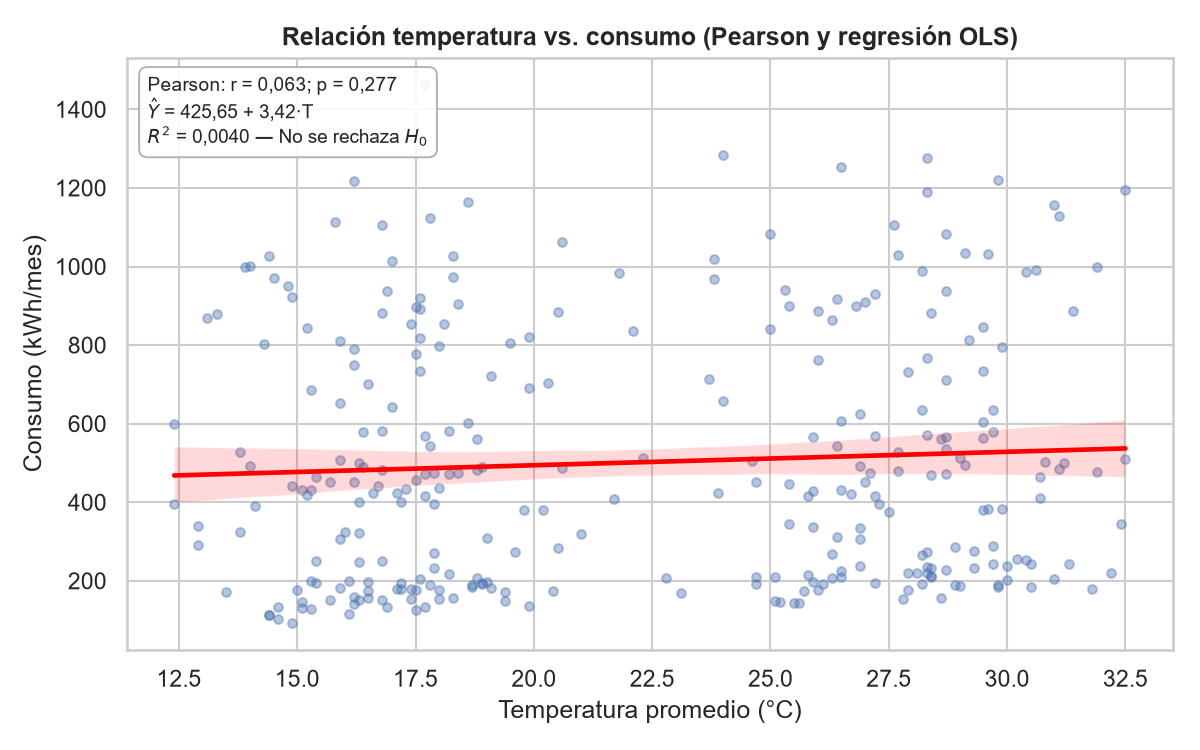
\includegraphics[width=1\linewidth]{assets/images/figures/python/hypothesis/regresion_temperatura.png}
            \caption{Relación temperatura-consumo sobre el conjunto agregado, con
            la recta de mínimos cuadrados, su banda de confianza y el resultado
            del contraste de Pearson rotulado (seaborn)}
            \label{fig_regresion}
        \end{figure}

        Acá se revela la contradicción, la nube se divide en tres franjas horizontales, 
        correspondientes a cada sector, mientras la recta global atraviesa las tres sin 
        representar adecuadamente a ninguna. La separación vertical entre franjas 
        responde al sector y no a la temperatura, dominando así la variabilidad 
        observada.
    \section{Conclusiones y recomendaciones}
    \begin{itemize}
        \item El protocolo de contraste confirmó que el sector determina el consumo
        energético de forma inequívoca, ya que el ANOVA atribuye el 83,9\,\% de la
        variabilidad a ese factor ($F = 775{,}99$; $p < 0{,}001$) y las tres
        comparaciones de Tukey resultan significativas, con diferencias de 244,3,
        456,4 y 700,7 kWh entre pares de sectores.

        \vspace{10pt}

        \item La verificación de supuestos no fue un trámite sino una decisión de
        método, puesto que el rechazo de la homogeneidad de varianzas obligó a
        emplear la corrección de Welch en la comparación de medias; omitir ese paso
        habría producido un valor $p$ calculado bajo un supuesto que los datos
        contradicen.

        \vspace{10pt}

        \item El incumplimiento de la homocedasticidad se resolvió contrastándolo y
        no advirtiéndolo, ya que repetir el análisis con el ANOVA de Welch
        ($F = 830{,}22$) y el post-hoc de Games-Howell reprodujo íntegramente la
        decisión del procedimiento clásico; la elección del método altera la
        precisión de cada intervalo, estrechándolo entre los sectores de menor
        varianza y ensanchándolo en los que involucran al Industrial, pero no la
        conclusión.

        \vspace{10pt}

        \item Reportar la magnitud junto al valor $p$ resultó indispensable para
        interpretar dos resultados que el estadístico presenta de forma engañosamente
        similar, dado que la diferencia entre sectores corresponde a un efecto
        enorme ($d = 3{,}33$; $\omega^2 = 0{,}838$) mientras que la correlación
        global no alcanza siquiera el umbral de $r_{\min} = 0{,}161$ detectable con
        potencia del 80\,\%, lo que descarta que su no significancia se deba a un
        tamaño muestral insuficiente.

        \vspace{10pt}

        \item El hallazgo central es que una prueba de hipótesis puede no rechazar
        $H_0$ aunque el efecto exista, ya que la correlación temperatura-consumo
        resulta no significativa a nivel agregado ($r = 0{,}063$; $p = 0{,}277$)
        pese a haberse introducido por diseño, y sí lo es dentro del sector
        Residencial ($r = 0{,}595$; $p < 0{,}001$).

        \vspace{10pt}

        \item El mecanismo de esa discrepancia quedó cuantificado mediante la
        relación $r = b_1 s_T / s_Y$, dado que la pendiente sobrevive a la
        agregación ($b_1 = 3{,}42$ frente al valor de diseño de 4) mientras la
        desviación estándar del consumo se triplica al mezclar sectores, de 40,6 a
        317,5 kWh, diluyendo la correlación sin alterar el efecto subyacente.

        \vspace{10pt}

        \item La visualización fue el instrumento que hizo visible esa estructura,
        puesto que la nube agregada de la Figura \ref{fig_regresion} muestra tres
        franjas horizontales atravesadas por una recta que no describe a ninguna,
        mientras que la figura interactiva de la Figura \ref{fig_plotly} revela tres
        pendientes positivas paralelas que ningún estadístico agregado permite
        anticipar.

        \vspace{10pt}

        \item La equivalencia entre Python y R, con coincidencia dígito a dígito en
        Shapiro-Wilk, la t de Welch, el ANOVA, Tukey, la regresión, los tamaños de
        efecto y ambos contrastes robustos, confirma que los resultados dependen de
        los datos y no de la herramienta; el acuerdo es especialmente exigente en
        Games-Howell y en la potencia, programados de cero en cada entorno a partir
        de sus fórmulas y no heredados de una biblioteca común.

        \vspace{10pt}

        \item Las nueve figuras se construyeron dos veces, con Matplotlib, seaborn y
        Plotly en Python y con ggplot2 en R, y cada una lleva impreso el estadístico
        que representa; las dos versiones interactivas y el tablero de cuatro paneles
        permiten además condicionar por sector sin recalcular nada, que es la
        operación exacta que separa la conclusión correcta de la equivocada.
    \end{itemize}

    \vspace{10pt}

    A partir de lo anterior se derivan tres recomendaciones para la toma de
    decisiones:

    \vspace{10pt}

    \begin{itemize}
        \item \textbf{Segmentar antes de promediar.} La media global de 501,98 kWh
        no describe a ningún cliente real, ya que se sitúa entre el sector Comercial
        y el Residencial sin representar a ninguno. Toda tarifa, meta de eficiencia
        o proyección de demanda debe construirse por sector, decisión que los
        intervalos de Tukey respaldan al excluir el cero con márgenes amplios y que
        descarta cualquier esquema tarifario de dos escalones.

        \vspace{10pt}

        \item \textbf{Incorporar la temperatura como variable de planeación
        únicamente en el segmento residencial.} Es el único donde la relación es a
        la vez significativa y de magnitud apreciable ($r = 0{,}595$), lo que la
        vuelve útil para anticipar picos de demanda en las regiones Caribe y
        Pacífica; extender esa conclusión al conjunto agregado carecería de
        sustento.

        \vspace{10pt}

        \item \textbf{Acompañar todo contraste con su representación gráfica antes
        de aceptar un resultado no significativo.} Este trabajo muestra que un valor
        $p$ elevado admite dos lecturas incompatibles, la ausencia de efecto y el
        enmascaramiento por agregación, que el estadístico no distingue y la figura
        sí. En conjuntos reales, donde la variable responsable de la agregación
        puede no estar registrada, esa inspección visual es la única salvaguarda
        disponible frente a una conclusión equivocada.
    \end{itemize}


    \appendices
    \section{Núcleo estadístico en Python}
    \label{anexo_python}
    Se reproduce el bloque de \textit{hypothesis\_testing.py} que implementa las
    cinco pruebas con \textit{SciPy} y \textit{statsmodels}. Se omiten la generación
    del conjunto de datos y el código de las figuras 1 a 4 por razones de extensión;
    el script completo está disponible en el repositorio del proyecto.

    \vspace{10pt}

    \lstinputlisting[style=python]{utils/codes/hypothesis_testing_core.py}

    \vspace{10pt}

    La figura interactiva de la Figura \ref{fig_plotly} se construye con
    \textit{Plotly Express}, cuyo argumento \texttt{trendline} delega el ajuste de
    la recta por grupo en \textit{statsmodels}, de modo que las pendientes de la
    Tabla \ref{atenuacion} y las dibujadas en la figura proceden del mismo cálculo.

    \vspace{10pt}

    \lstinputlisting[style=python]{utils/codes/plotly_figure.py}

    \section{Código en R}
\label{r_code}
    El script de R implementa la verificación cruzada del análisis, pues lee el mismo
    archivo CSV generado en Python, recalcula de forma independiente las medias
    sectoriales, las participaciones y la correlación entre consumo y costo, y replica
    con la graficación base las Figuras \ref{r_replicas_good} y
    \ref{r_replicas_share}, trazando la cuadrícula en dos pasadas para mantenerla por
    detrás de los datos.

    \vspace{10pt}

    \lstinputlisting[style=Rstyle]{utils/codes/r/visualizations.R}


    \bibliographystyle{IEEEtran}
    \bibliography{utils/references/references.bib}
\end{document}
